\documentclass[border=2cm]{standalone}
\usepackage[T1]{fontenc}
\usepackage[tt=false, type1=true]{libertine}
\usepackage[varqu]{zi4}
\usepackage{subcaption}
\usepackage{graphicx}
\usepackage[font=bf]{caption}
\usepackage{listings}
\pagestyle{empty}

\lstset{
  basicstyle=\small\ttfamily,
  keywordstyle=\textbf,
  breaklines=true,
  numbers=left,
  morekeywords={Subquery,Scan,WindowAgg,Sort,Bitmap,Heap,Index,Gather,Merge,Parallel,Seq,Scan,Unique},
  deletekeywords={on},
  columns=fullflexible
}

\let\IG\includegraphics
\renewcommand\includegraphics[2][]{
  \IfFileExists{#2}{
    \IG[#1]{#2}
  }{
      \fbox{\textit{Missing figure}}
  }
}

\let\LIL\lstinputlisting
\renewcommand\lstinputlisting[1]{
  \IfFileExists{#1}{
    \LIL{#1}
  }{
      \centering
      \fbox{\textit{Missing file}}
  }
}

\begin{document}

\begin{minipage}{17cm}

  \setcounter{section}{4}
  \setcounter{figure}{5}
  \setcounter{lstlisting}{2}

  \section{Evaluation}

  \begin{figure}[t]
    \centering
    \begin{subfigure}{0.5\textwidth}
      \centering
      \hspace*{0.7cm}
      
\includegraphics[width=0.74\textwidth]{../results/plots/te_legend.pdf}
    \end{subfigure}

    \medskip

    \begin{subfigure}{.26\textwidth}
      \centering
      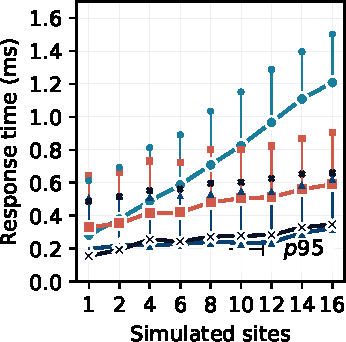
\includegraphics[width=\textwidth]{../results/plots/te_currTime.pdf}
      \subcaption{Current time}
      \label{fig:te_curr}
    \end{subfigure}
    \hspace*{0.5cm}
    \begin{subfigure}{.26\textwidth}
      \centering
      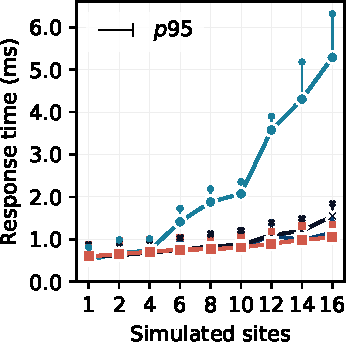
\includegraphics[width=\textwidth]{../results/plots/te_readKey.pdf}
      \subcaption{Causal present}
      \label{fig:te_read}
    \end{subfigure}
    \par\bigskip
    \begin{subfigure}{.26\textwidth}
      \centering
      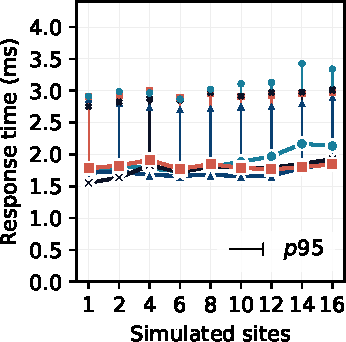
\includegraphics[width=\textwidth]{../results/plots/te_write.pdf}
      \subcaption{Write}
      \label{fig:te_write}
    \end{subfigure}
    \hspace*{0.5cm}
    \begin{subfigure}{.26\textwidth}
      \centering
      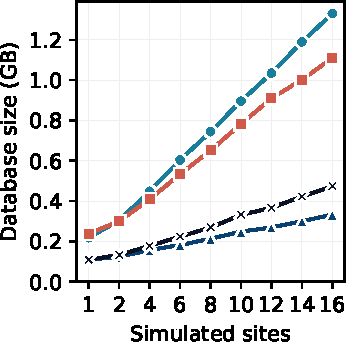
\includegraphics[width=\textwidth]{../results/plots/te_size.pdf}
      \subcaption{Size}
      \label{fig:te_size}
    \end{subfigure}
    \caption{Comparison of different timestamp encodings.}
    \label{fig:te}
  \end{figure}

  \medskip

  \begin{figure}[t]
    \centering
    \begin{subfigure}[T]{.23\linewidth}
      \centering
      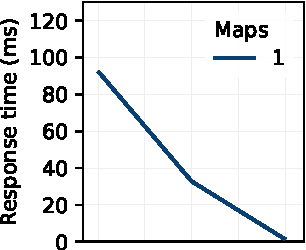
\includegraphics[width=\linewidth]{../results/plots/materialization_rt_sync.pdf}
      \label{fig:materialization_rt_sync}
    \end{subfigure}
    \begin{subfigure}[T]{.1687\linewidth}
      \centering
      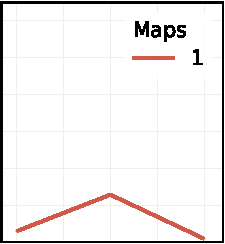
\includegraphics[width=\linewidth]{../results/plots/materialization_rt_async.pdf}
      \label{fig:materialization_rt_async}
    \end{subfigure}
    \begin{subfigure}[T]{.1687\linewidth}
      \centering
      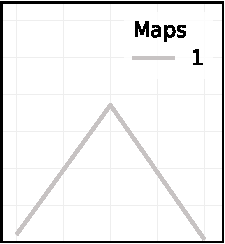
\includegraphics[width=\linewidth]{../results/plots/materialization_rt_no-mat.pdf}
      \label{fig:materialization_rt_nomat}
    \end{subfigure}
    \\[-0.45cm]
    \begin{subfigure}[T]{.23\linewidth}
      \centering
      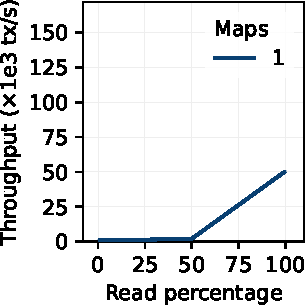
\includegraphics[width=\linewidth]{../results/plots/materialization_tps_sync.pdf}
      \subcaption{\textit{Sync}}
      \label{fig:materialization_tps_sync}
    \end{subfigure}
    \begin{subfigure}[T]{.1687\linewidth}
      \centering
      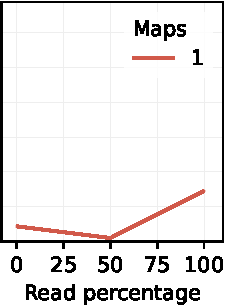
\includegraphics[width=\linewidth]{../results/plots/materialization_tps_async.pdf}
      \subcaption{\textit{Async}}
      \label{fig:materialization_tps_async}
    \end{subfigure}
    \begin{subfigure}[T]{.1687\linewidth}
      \centering
      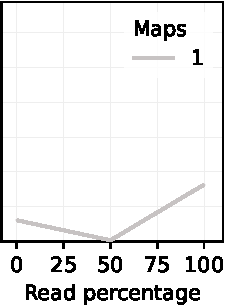
\includegraphics[width=\linewidth]{../results/plots/materialization_tps_no-mat.pdf}
      \subcaption{\textit{No-mat}}
      \label{fig:materialization_tps_nomat}
    \end{subfigure}
    \caption{Comparison of different materialization strategies in CRDV, based on the workload and number of \textit{maps}.}
    \label{fig:materialization}
  \end{figure}

  \medskip

  \begin{figure}[t]
    \centering
    \begin{subfigure}{0.5\linewidth}
      \lstinputlisting{../results/plans/plan1.txt}
      \caption{\texttt{WHERE cart\_id = $x$}}
    \end{subfigure}

    \begin{subfigure}{0.42\linewidth}
      \lstinputlisting{../results/plans/plan2.txt}
      \subcaption{\texttt{WHERE p\_id BETWEEN $x$ AND $y$}}
    \end{subfigure}
    \hspace{1cm}
    \begin{subfigure}{0.42\linewidth}
      \lstinputlisting{../results/plans/plan2opt.txt}
      \subcaption{b) + an index on \texttt{p\_id}}
    \end{subfigure}
    \captionof{lstlisting}{Physical plans for different CRDV queries}
    \label{fig:plan_optimization}
  \end{figure}


  \medskip

  \begin{figure}[t]
    \centering
    \begin{subfigure}{.26\linewidth}
      \centering
      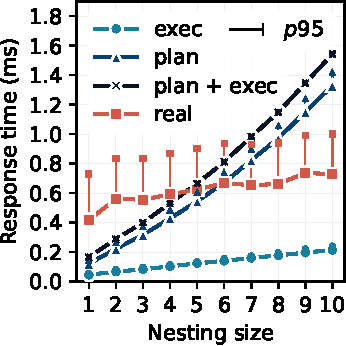
\includegraphics[width=\linewidth]{../results/plots/nested.pdf}
      \subcaption{Response time}
      \label{fig:nested_latency}
    \end{subfigure}
    \nextfloat
    \caption{CRDV's read performance with different levels of nesting.
      \small \normalfont $M$ refers to the \textit{MapAwLww} view.}
    \label{fig:nested}
  \end{figure}

  \medskip

  \begin{figure}[t]
    \centering
    \begin{minipage}{\textwidth}
      \centering
      \hspace*{0.7cm}
      
\includegraphics[width=0.65\textwidth]{../results/plots/operations_legend.pdf}
      \smallskip
    \end{minipage}
    \subfloat[Register]{
      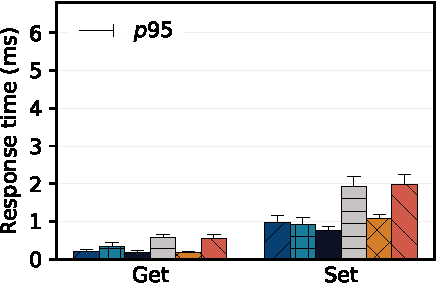
\includegraphics[height=2.6cm]{../results/plots/operations_register.pdf}
      \label{fig:operations_register}
    }
    \subfloat[Counter]{
      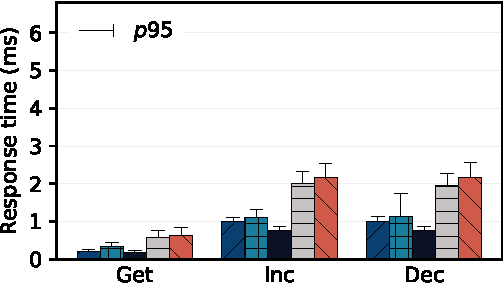
\includegraphics[height=2.6cm]{../results/plots/operations_counter.pdf}
      \label{fig:operations_counter}
    }
    \subfloat[Set]{
      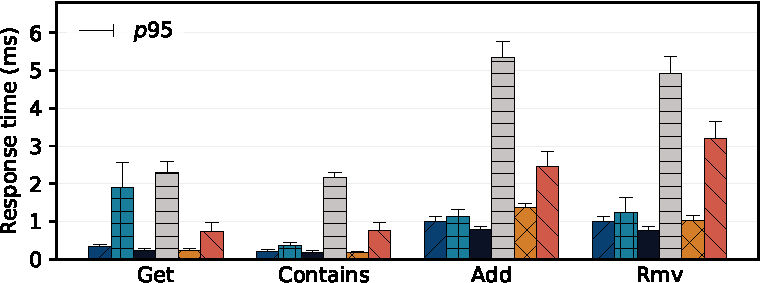
\includegraphics[height=2.6cm]{../results/plots/operations_set.pdf}
      \label{fig:operations_set}
    }\\[0.15cm]
    \subfloat[List]{
      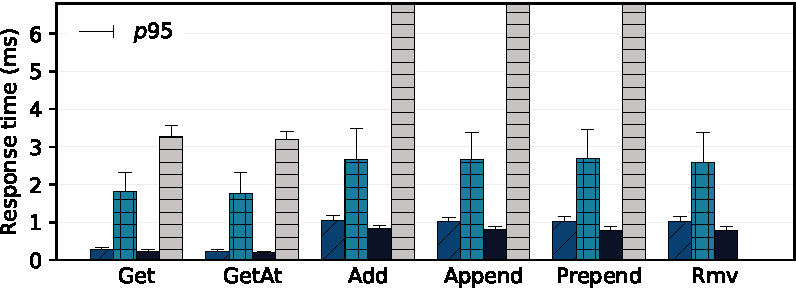
\includegraphics[height=2.6cm]{../results/plots/operations_list.pdf}
      \label{fig:operations_list}
    }
    \subfloat[Map]{
      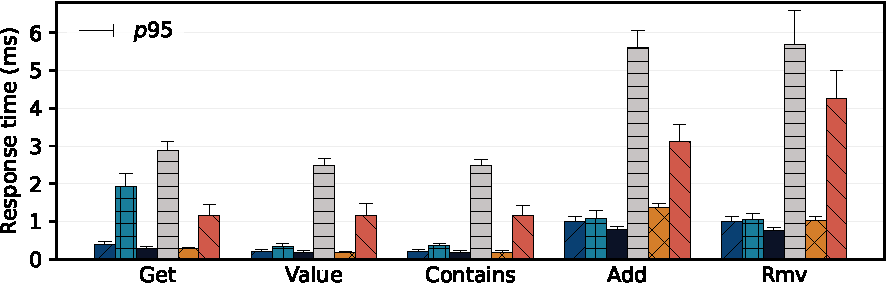
\includegraphics[height=2.6cm]{../results/plots/operations_map.pdf}
      \label{fig:op_map}
    }
    \caption{Performance comparison between different operations in different structures, using different solutions.
      \small \normalfont \textit{Get} - read the structure; \textit{GetAt} - list's element at some index; \textit{Contains} - check if an element/key exists in a \textit{set}/\textit{map}; \textit{Value} - value of some key in a \textit{map}; \textit{Set} - update a \textit{register}; \textit{Inc/Dec} - increment/decrement a counter; \textit{Add} - add a new entry to a \textit{set}/\textit{list}/\textit{map} or update a \textit{map's} value; \textit{Prepend/Append} - insert an entry at the start/end of a list; \textit{Rmv} - remove an entry from a \textit{set}/\textit{list}/\textit{map}. The missing structures/operations are not supported by their respective solutions.}
    \label{fig:op}
  \end{figure}

  \medskip

  \begin{figure}[t]
    \centering
    \begin{subfigure}{\linewidth}
      \centering
      \hspace*{0.8cm}
      
\includegraphics[width=0.65\linewidth]{../results/plots/concurrency_legend.pdf}
    \end{subfigure}

    \medskip

    \begin{subfigure}{.26\linewidth}
      \centering
      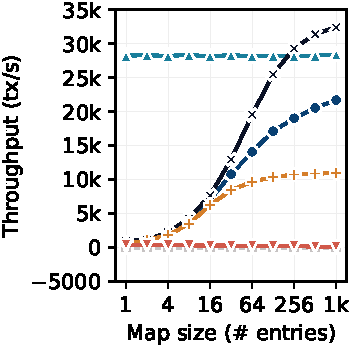
\includegraphics[width=\linewidth]{../results/plots/concurrency_tps.pdf}
      \subcaption{Throughput}
      \label{fig:concurrency_tps}
    \end{subfigure}
    \hspace*{0.5cm}
    \begin{subfigure}{.26\linewidth}
      \centering
      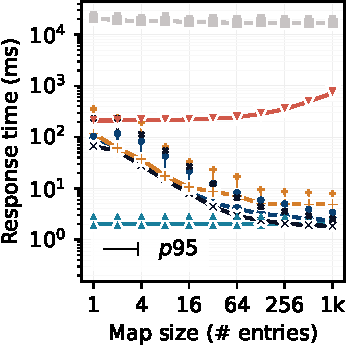
\includegraphics[width=\linewidth]{../results/plots/concurrency_rt.pdf}
      \subcaption{Response time}
      \label{fig:concurrency_rt}
    \end{subfigure}
    \caption{Write performance of different solutions in a variable contention workload, using 64 clients.}
    \label{fig:concurrency}
  \end{figure}

  \medskip

  \begin{figure}[t]
    \centering
    \begin{subfigure}{\linewidth}
      \centering
      \hspace*{0.8cm}
      
\includegraphics[width=0.65\linewidth]{../results/plots/storage_legend.pdf}
    \end{subfigure}

    \medskip

    \begin{subfigure}{.22\linewidth}
      \centering
      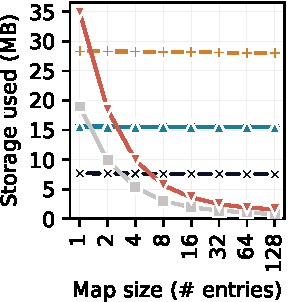
\includegraphics[width=\linewidth]{../results/plots/storage.pdf}
      \subcaption{Storage}
      \label{fig:storage_mb}
    \end{subfigure}
    \hspace*{0.5cm}
    \begin{subfigure}{.173\linewidth}
      \centering
      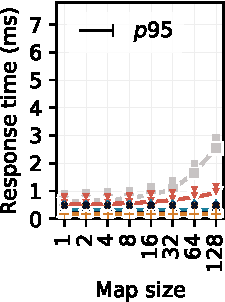
\includegraphics[width=\linewidth]{../results/plots/storage_rt_read.pdf}
      \subcaption{Reads}
      \label{fig:storage_read}
    \end{subfigure}
    \begin{subfigure}{.1315\linewidth}
      \centering
      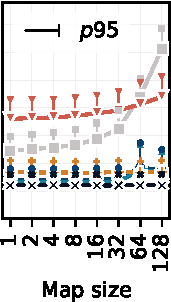
\includegraphics[width=\linewidth]{../results/plots/storage_rt_write.pdf}
      \subcaption{Writes}
      \label{fig:storage_write}
    \end{subfigure}
    \caption{Storage usage and latency of different solutions with 100k key-value pairs, based on the total number of \textit{maps}.
      \normalfont \small $x \! = \! 1 \rightarrow 100\mbox{k}$ \textit{maps} of size 1, $x \! = \! 2 \rightarrow 50\mbox{k}$ \textit{maps} of size 2, and so on.}
    \label{fig:storage}
  \end{figure}

  \medskip

  \begin{figure}[t]
    \centering
    \begin{subfigure}{.26\linewidth}
      \centering
      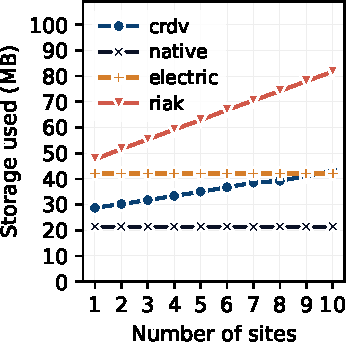
\includegraphics[width=\linewidth]{../results/plots/storage_sites.pdf}
      \subcaption{Total storage per site}
      \label{fig:storage_sites_mb}
    \end{subfigure}
    \caption{Storage usage based on the number of sites.}
    \label{fig:storage_sites}
  \end{figure}

  \medskip

  \begin{figure}[t]
    \centering
    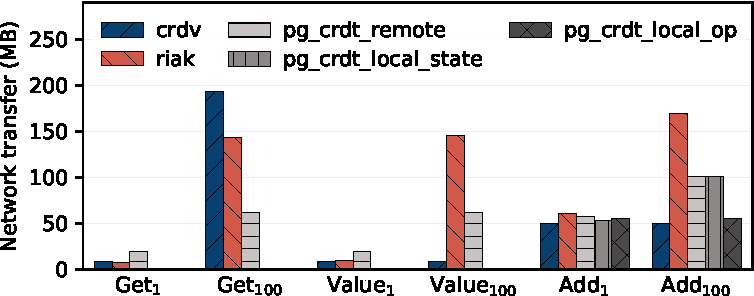
\includegraphics[width=0.55\linewidth]{../results/plots/network_map.pdf}
    \caption{Network overhead of different distributed solutions, based on 100k operations performed to \textit{maps}.
      \normalfont \small $X_1$ and $X_{100}$ represent operations done to \textit{maps} with $1$ and $100$ entries, respectively.}
    \label{fig:network}
  \end{figure}

  \medskip

  \begin{figure}[t]
    \centering
    \begin{subfigure}[T]{\linewidth}
      \centering
      \hspace*{0.95cm}
      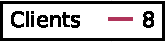
\includegraphics[width=0.41\linewidth]{../results/plots/freshness_legend.pdf}
    \end{subfigure}

    \smallskip

    \begin{subfigure}[T]{.225\linewidth}
      \centering
      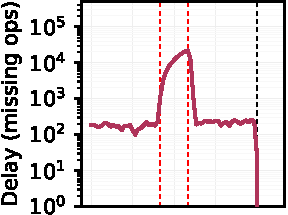
\includegraphics[width=\linewidth]{../results/plots/freshness_crdv.pdf}
    \end{subfigure}
    \begin{subfigure}[T]{.163\linewidth}
      \centering
      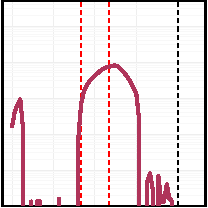
\includegraphics[width=\linewidth]{../results/plots/freshness_riak.pdf}
    \end{subfigure}
    \begin{subfigure}[T]{.163\linewidth}
      \centering
      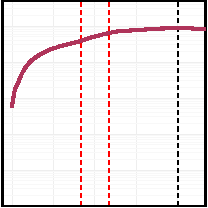
\includegraphics[width=\linewidth]{../results/plots/freshness_pg_crdt.pdf}
    \end{subfigure}
    \\[-0.4cm]
    \begin{subfigure}[T]{.225\linewidth}
      \centering
      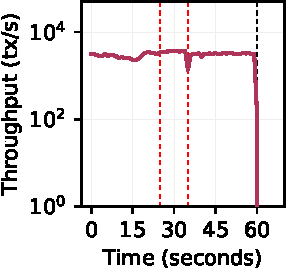
\includegraphics[width=\linewidth]{../results/plots/freshness_tps_crdv.pdf}
      \subcaption{CRDV}
      \label{fig:delay_crdv}
    \end{subfigure}
    \begin{subfigure}[T]{.163\linewidth}
      \centering
      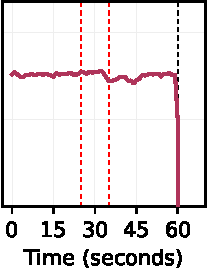
\includegraphics[width=\linewidth]{../results/plots/freshness_tps_riak.pdf}
      \subcaption{Riak}
      \label{fig:delay_riak}
    \end{subfigure}
    \begin{subfigure}[T]{.163\linewidth}
      \centering
      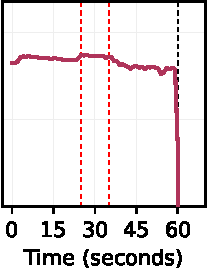
\includegraphics[width=\linewidth]{../results/plots/freshness_tps_pg_crdt.pdf}
      \subcaption{Pg\_crdt(\textit{local op})}
      \label{fig:delay_pgcrdt}
    \end{subfigure}
    \nextfloat
    \caption{Delay and throughput over time of different distributed solutions.
      \normalfont \small The network is partitioned between t=25 and t=35.}
    \label{fig:freshness}
  \end{figure}

  \medskip

  \begin{figure}[t]
    \centering
    \begin{subfigure}{\linewidth}
      \centering
      \hspace*{1.1cm}
      
\includegraphics[width=0.4\linewidth]{../results/plots/sites_legend.pdf}
    \end{subfigure}

    \smallskip

    \begin{subfigure}{.26\linewidth}
      \centering
      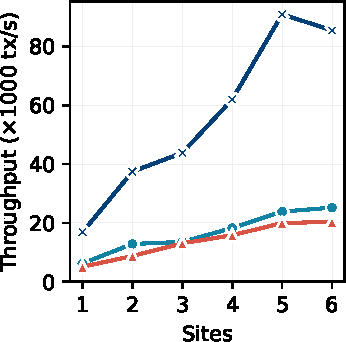
\includegraphics[width=\linewidth]{../results/plots/sites_r.pdf}
      \subcaption{Reads}
      \label{fig:sites_read}
    \end{subfigure}
    \hspace*{0.5cm}
    \begin{subfigure}{.26\linewidth}
      \centering
      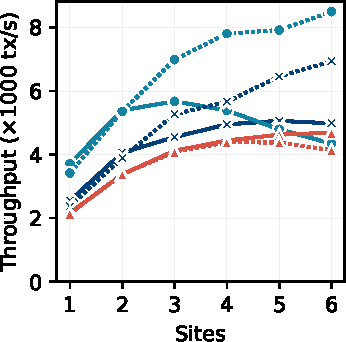
\includegraphics[width=\linewidth]{../results/plots/sites_w.pdf}
      \subcaption{Writes}
      \label{fig:sites_write}
    \end{subfigure}
    \nextfloat
    \caption{Performance comparison based on the cluster size.}
    \label{fig:scale}
  \end{figure}


\end{minipage}

\end{document}
